\section{Artificial Intelligence}
As mentioned earlier, there is no scripting language is \doom. The A.I is based on a per enemy type state machine which is backed inside the engine binary. Designers did not have learn C however since they could entirely configure an opponent via a text file \cw{multigen.txt} which is parsed by a tool (cunningly named \cw{multigen}) and compiled into a C structure (\cw{info.h} and \cw{info.c}).\\
\par
\rawdrawing{multigen}
\par
% The script has two sections per entity. First the general info and then a serie of state machines. To illustrate here if the imp script.\\
For once, let's dive into the text code right away and take a look at the section of \cw{multigen.txt}  which describe the Imp (known as \cw{TROOP} internaly).\\
\par
\tcode{enemy_info.txt}

\tcode{imp_state.txt}

There are four sections. Properties such as DoomED id, \cw{speed}, \cw{heigh}, \cw{radius}. State names for state machine targets. Sound strings. And finally the huge State definition.






Properties list and sound names are self-explanatory, no need to spend too much time on it. What is more difficult to understand is how the state machine is defined.\\
\par
A thing state machine is partly statically defined inside the engine (when a monster is attacked it goes directly to \cw{seestate}) and partly defined in \cw{multigen.txt}. Each line is the state defintion follows a syntax.
\begin{enumerate}
\item State name.
\item Frame family.
\item Frame ID (sprite to render).
\item Duration in tics (engine runs 35 tics/seconds).
\item Function to call when in this state.
\item Next state.
\end{enumerate}
\par
Let's take the example of an Imp which was just spawned in a level and therefore is in state \cw{spawnstate} which is \cw{S\_TROO\_STND}. Upon simulating each game tic, the engine looks at what to do in this state. In this case, the Imp will cycle between state action \cw{S\_TROO\_STND} and \cw{S\_TROO\_STND2}. In these sub-states, \cw{A\_Look} is called each tics trying to detect the player. If it does, the engine place the imp in \cw{seestate} (a.k.a S\_TROO\_RUN1)\\
\par

Now this Imp was unlucky, the player was fast and managed to hit with a shotgun at point blank. In this case the engine place the Imp in the Imp's \cw{deathstate} (\cw{S\_TROO\_DIE1}).\\
\par
\tcode{enemy_state_die.txt}\\
\par

\fullimage{imp_die}
\par


\pagebreak
Let's follow the chain of state from here, where an imp dies in five steps.

\begin{enumerate}
\item Show first death frame (I) for 8/35th of a second.
\item Show second death frame (J) for 8/35th of a second. Scream using \cw{deathsound}.
\item Show third death frame (K) for 6/35th of a second.
\item Show fourth death frame (L) for 6/35th of a second. Mark itself as non-obstacle (\cw{FALL}).
\item Show fifth death frame (M) forever (\cw{-1}).
\end{enumerate}
\par
The total dying sequence lasts $8+8+6+6=24/35 = 0.68$ second. Note that this Imp could have been even less lucky and bit hit by a rocket. Enough damage would have gibbed it into \cw{xdeathstate} (\cw{S\_TROO\_XDIE1}) state and made it die in $1$ second.\\
\par
\tcode{enemy_state_xdie.txt}\\
\par
\fullimage{imp_xdie}




\par
\begin{wrapfigure}[9]{r}{0.25\textwidth}
\centering

\includegraphics[width=.25\textwidth]{drawings/sprite_quantization.pdf}
\end{wrapfigure}
The engine uses a convention to find what sprite to use when rendering them. Because an enemy will not always be facing the player, it uses quantization where all orientation with regard to the player position fall into eight cases (see drawing where 1 is facing player, 5 back to player and so on).\\
\par
When in \cw{S\_TROO\_XDIE1} state, according to \cw{multigen.txt}, the engine must use sprite family \cw{TROO} and frame \cw{N}. Based on the orientation (lets say the Imp is back to the player), the engine should use \cw{TROON5}. But since these is no such sprite in \cw{DOOM.WAD} (exploding enemies always face the player) the engine falls back to \cw{TROONO} (0 being the "always facing" sprite).
\par







\cfullimage{cyber_sprite}{CyberDemon poses in one of its two "walk" position}
\par
Taking a look at one of the frame for the Cyberdemon in figure \ref{cyber_sprite} give a good idea of the collosal work requiered from artists. Twelve monsters times eight states times average of five frames per animation would have required close to 480 drawings (for the monsters only). The power of the NextDimension made a tremendous different in this department.\\
\par
The cyberdemon however is an extreme case since it is not symetric. Imps sprite storage is optimized to take advantage of its symetry. If the engine needs \cw{TROOA6} but doesn't find it in the \cw{WAD}, it uses its opposite (\cw{TROOA4}) and draws it horizontally inverted. 
\par
\trivia{You may have noticed in the list of state, a non obvious one named \cw{RAISE}. It is used when the Arch-vile enemy resurrects a dead monsters. The animation plays the dying frame in reverse. Not that there are no reverse gibing so Arch-vile doesn't revive gibbed monsters.}




\begin{figure}[H] \centering
\cscaledimage{0.9}{imp_sprite}{}
\end{figure}
\par
\trivia{When an entity receives more than  \cw{spawnhealth} damage (negative its spawing state, in the case of an imp that would be -60), the engine triggers not \cw{deathstate} but \cw{xdeathstate} state which means the entity exploded.}\\
\par 
\ccode{explode.c}\\
\par





\cw{multigen.txt} is compiled to an humongus 5000 lines \cw{info.c} made of an array of \cw{state\_t} holding the state machine and an array of \cw{mobjinfo\_t} holding the things properties.\\
\par
\ccode{enemy_state_compiled.c}\\
\par
To lighten the load of monster sight awakening, maps feature a \cw{REJECT} lump with contains a precalculated list of sectors visible by each monsters in startup position.\\
\par
\rawdrawing{E1M1_sides}
% Regardless of the monsters, the base state machine looks like this but it tuned based on custom functions called in some states (e.g: \cw{A\_SpidRefire}, \cw{A\_CyberAttack}, and \cw{A\_BrainExplode}).\\
% \par
% \pngdrawing{automate}{}
\pagebreak






\section{Map Intelligence}
Despite lacking a scripting system, maps still managed to offer a rich experience. Maps were full of surprises with elements interacting with the player. Switches and trip wire enabled door, secret passages, elevators, crushing walls, traps and many others.\\
\par
\pngdrawing{tripwire}{E1M1 features no less than XX special lines}
\par
All effects are achieved via lines \cw{special} attribute which designate an action and \cw{tag} which is the action parameter (usually a sector tag).\\
\par
The list of types of actions is impressive, there are more than 130 of them. Open/Close door normal/turbo/blazing speeds. Raise/Lower floor and ceilings, Fast Ceiling Crush \& Raise, Build Stairs, Lock door so you are trapped with monsters, Change light levels, Raise floor to nearest height and change texture, teleport, Exit level, Secret exit,  .\\
\par
Target. Note that several sector can have the same tag so a line can have only one type of action but target multiple sectors.\\
\par
Thinkers injection\\
\par
Studying the architecture of the maps really make apprecite the amount of effort that went into them. Dongons \& Dragons background.
\pagebreak






\begin{wrapfigure}[17]{r}{0.5\textwidth}
\centering
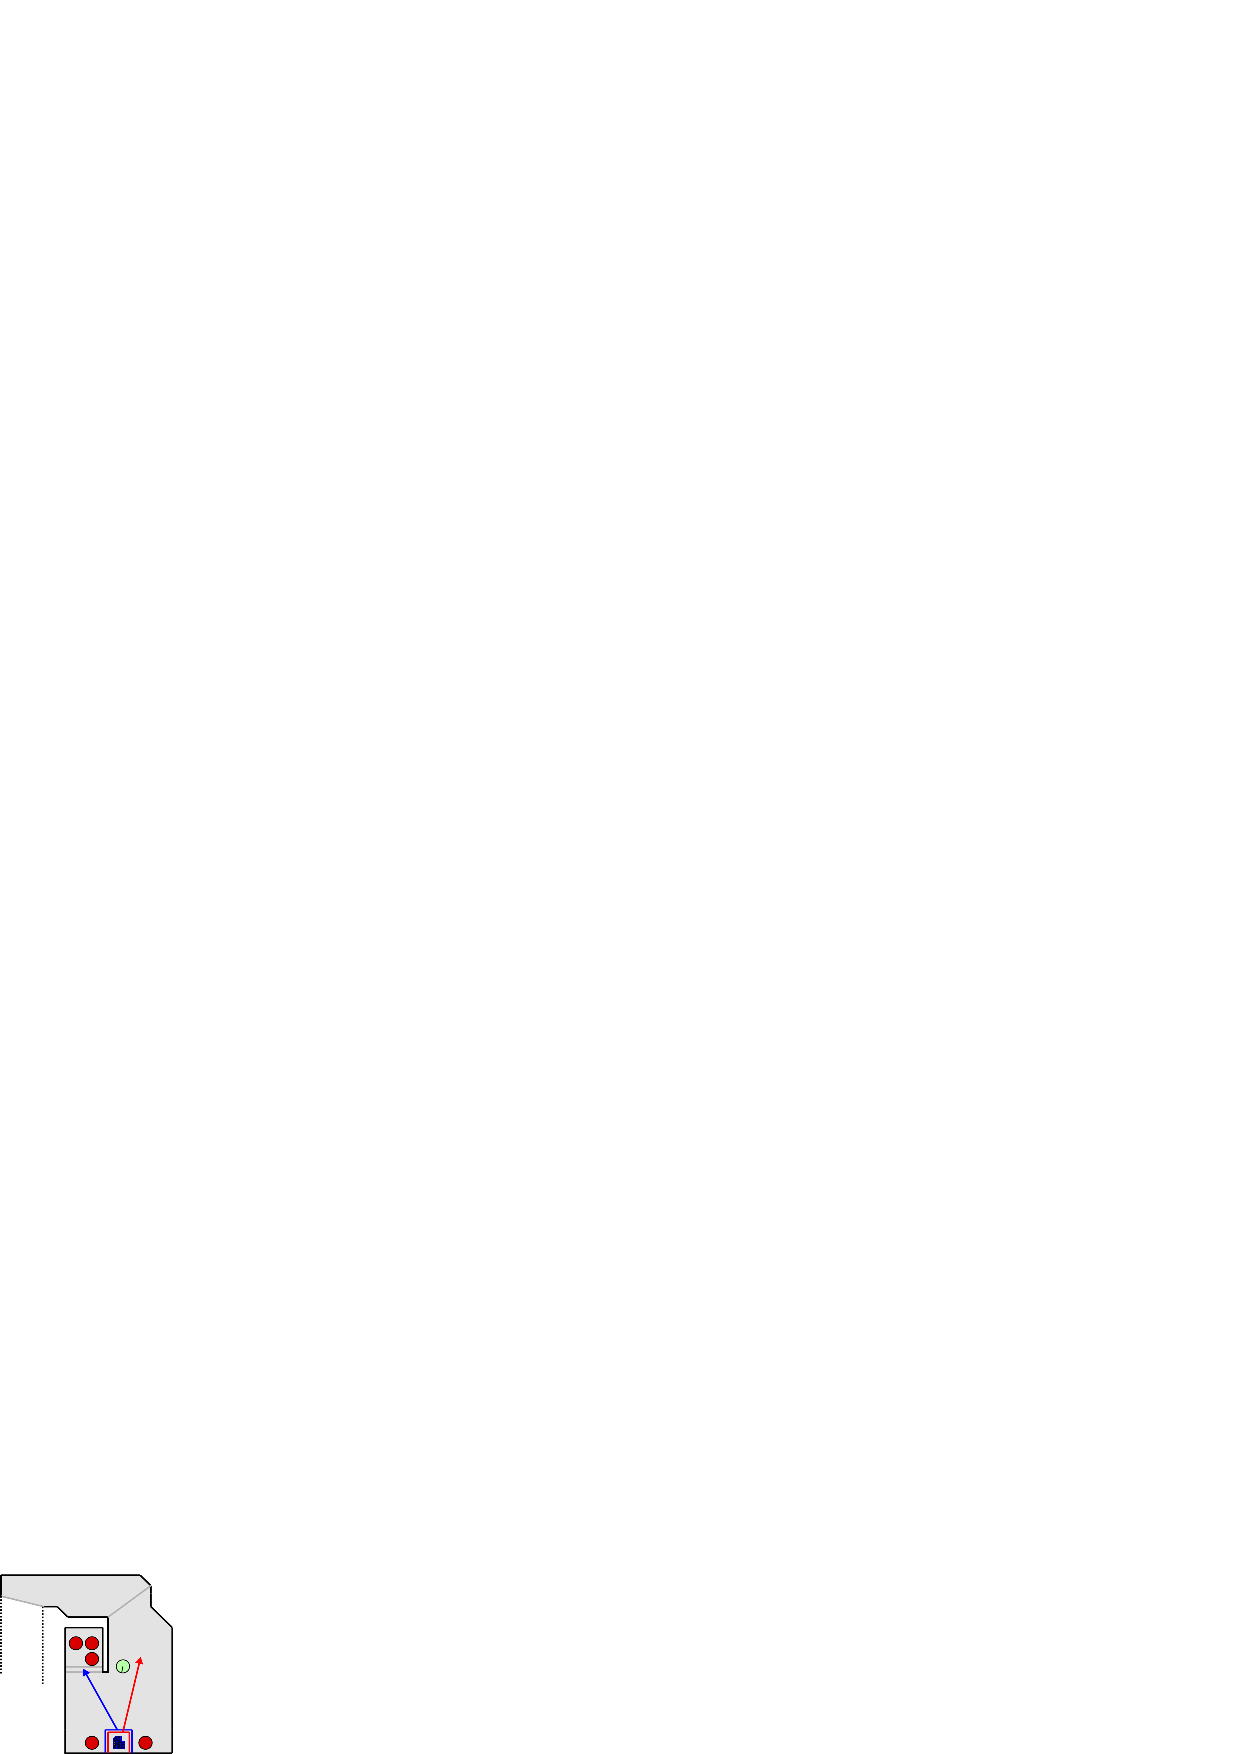
\includegraphics[width=.5\textwidth]{drawings/E1M3_trap.pdf}
\end{wrapfigure}
Who doesn't recognize E1M3 hunt for the blue key (figure \ref{Doom-E1M3-Ingame2.png}). After traversing the full level, it is finally there enlighted on a pedestral. Guarded by only two low levels opponents which are easily dispatched.\\
\par
But as soon as the player picks it up, all light go off and the combined sound of a door opening and growling Imps leaves no doubt: It was trap and Imps are just behind (figure \ref{Doom-E1M3-Ingame3.png})!\\
\par
To implement this effects, two set of lines were used. The first one (in blue) targets the door sector via tag YY where the monsters were hiding. Action XX opens it. The second one (in red) targets the current sector via tag XX and set the light level to "very dark".\\
\par
\cfullimage{e4m6.png}{E4M6 few AA lines and many triggers make you appreciate the collosal effort of map design.}






\pagebreak
\cfullimage{Doom-E1M3-Ingame2.png}{Finally, the blue key!}
\par
\cfullimage{Doom-E1M3-Ingame3.png}{It's a TRAP!}

\pagebreak
\section{Game tics Architecture}
With knownledge of how opponents and map elements work, we can pickup the code where we had left it with regard to game simulation on page \pageref{TryRunTics.c}. \cw{G\_Ticker} is where all thinkers tic. \cw{P\_Ticker} is where most of the 3D action is.\\
\par
\ccode{G_Ticker.c}
\par
Actors are organized as "Thinkers".\\
\par
\ccode{P_Ticker.c}
